\chapter*{mods}
Our game allows you to alter some of its properties and content. This manual only describes the modding possibilities. For a more technical description, please refer to the docs inside our git repository. 

\section*{ship graphics}
In the game two different ship models are used. One for the mothership and one for the fleep. They consist of different detail layers. You can swap each layer with your own images and will be loaded on next client start. For the detail image you can either provide a single image or generate different frames and combine them into an animted gif. The default in-game models (all frames shown) look like this:

\subsection*{mothership}

\begin{figure}[!htb]
\minipage{0.15\textwidth}%
  
\includegraphics[width=\linewidth]{chapters/modding/shipBody.png}
  \caption*{Body Detail}
\endminipage\hfill
\minipage{0.15\textwidth}%
  
\includegraphics[width=\linewidth]{chapters/modding/shipDetails_1.png}
  \caption*{Frame 1}
\endminipage\hfill
\minipage{0.15\textwidth}%
  
\includegraphics[width=\linewidth]{chapters/modding/shipDetails_2.png}
  \caption*{Frame 2}
\endminipage\hfill
\minipage{0.15\textwidth}%
  
\includegraphics[width=\linewidth]{chapters/modding/shipDetails_3.png}
  \caption*{Frame 3}
\endminipage\hfill
\end{figure}
\newpage
\subsection*{fleet ships}

\begin{figure}[!h]
\minipage{0.15\textwidth}%
  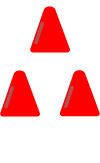
\includegraphics[width=\linewidth]{chapters/modding/fleetBody.png}
  \caption*{Body Detail}
\endminipage\hfill
\minipage{0.15\textwidth}%
  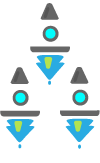
\includegraphics[width=\linewidth]{chapters/modding/fleetDetails_3.png}
  \caption*{Frame 1}
\endminipage\hfill
\minipage{0.15\textwidth}%
  
\includegraphics[width=\linewidth]{chapters/modding/fleetDetails_2.png}
  \caption*{Frame 2}
\endminipage\hfill
\minipage{0.15\textwidth}%
  
\includegraphics[width=\linewidth]{chapters/modding/fleetDetails_1.png}
  \caption*{Frame 3}
\endminipage\hfill
\end{figure}

\section*{star names}
All the names for the stars are read from a huge list. You can supply your own names if you'd like. To do so create a UTF-8 encoded texfile in the \textbf{config/mods/stars/} folder. The first line needs to contain an integer which represents the weight of the textfile. The higher the number, the more likely the names are picked from this file. The biggest number in the default lists is 999. You can provide as many files as you want. Example:

\begin{Verbatim}[numbers=left,xleftmargin=6mm]
  ## config/mods/stars/modded-stars.txt
  999999
  starname 1
  starname 2
  ...
  ...
  starname n-1
  starname n
  # EOF
\end{Verbatim}

\section*{chatbots}
The chat component features support for simple chatbots written in javascript. Bots need to be placed in the folder \textbf{config/mods/chatbots/}. The name of the file will also be the name of your bot. Use the \textbf{>} symbol to talk to a chatbot. A \emph{cat} bot (just echos whatever argument you give it) and a \emph{list} bot (lists all available bots) are already part of the game. For example a bot that rolls an n-sided dice and prints the outcome to the chat could like this:

\begin{Verbatim}[numbers=left,xleftmargin=6mm]
  ## config/mods/chatbots/roll.js
  function(msg, reply, replyAll) {
      var sides = parseInt(msg) || 6;
      var res = Math.floor(Math.random() * sides) + 1;
      replyAll('you rolled a ' + res);
  }
  # EOF

  ## Usesage
  you: >roll 20
  roll: you rolled a 16
\end{Verbatim}